
\documentclass[11pt, oneside]{article}   	% use "amsart" instead of "article" for AMSLaTeX format
\usepackage{geometry}                		% See geometry.pdf to learn the layout options. There are lots.
\geometry{letterpaper}                   		% ... or a4paper or a5paper or ... 
%\geometry{landscape}                		% Activate for rotated page geometry
%\usepackage[parfill]{parskip}    		% Activate to begin paragraphs with an empty line rather than an indent
\usepackage{amsmath}\usepackage{graphicx}				% Use pdf, png, jpg, or eps§ with pdflatex; use eps in DVI mode
\usepackage{tikz}								% TeX will automatically convert eps --> pdf in pdflatex		
\usepackage{amssymb}
\usepackage{subcaption}%SetFonts

%SetFonts


\title{Lecture Note }
\author{Yiping Lu, Jody Shu and Jashaina Thomas}
%\date{}							% Activate to display a given date or no date

\begin{document}
\maketitle
%\section{}
%\subsection{}

 \textbf{\Large Recall}\\
 \\
 \begin{Large}
     P(t)   $\leftarrow$ price\\
     V(t)   $\leftarrow$ volume\\
     S(t)   $\leftarrow$ sensitivity\\
     C(t)   $\leftarrow$ cash flow\\
     Sh(t) $\leftarrow$ sharpe ratio\\
     \vdots\\
     many more\\
     \\
  ${\Large N\choose K}$\\   
  

\begin{figure}[htbp]

\begin{tikzpicture}

\draw (1,0) -- (0,0) -- (0,1);
\node at (1,0) [right]  {$P$};
\node at (0,1) [left] {$V$}      ;
\end{tikzpicture}
\end{figure}

${\Large N\choose 2}$\\
\begin{figure}[htbp]
\begin{tikzpicture}
\draw (0,0) -- (-0.5,-0,2);
\draw (1,0) -- (0,0) -- (0,1);
\node at (1,0) [right]  {$P$};
\node at (0,1) [left] {$S$};
\node at (-0.5,-0.2)[left]{$V$};
\end{tikzpicture}
\end{figure}
\\
${\Large N\choose 3}$\\\\

$X_i=\frac{P_i -P_{i-1}}{P_i} ,  P_i=P(t_i)$ ,
$Y_i=\frac{V_i -V_{i-1}}{V_i},  V_i=V(t_i)$ \\

\[
   X=
  \left[ {\begin{array}{cc}
   x_1 & y_1 \\
   x_2&  y_2 \\
   \vdots &\vdots\\
   x_n & y_n
  \end{array} } \right]
\]\\
Consider  $\mathbf{X}^T\mathbf{X}$ and  $\mathbf{XX}^T$ $\leftarrow$  We orthogonally diagonalize them.\\
 
Let $\mathbf{A_{2x2}}=\mathbf{X}^\top\mathbf{X} \Rightarrow $there exists orthogonal matrix $P_{2x2}$ such that\\
\\
\hspace{40pt}$\mathbf{P}^\top\mathbf{A}\mathbf{P}=\mathbf{D}$=
$\begin{pmatrix}
\lambda_1 & 0\\
0 & \lambda_2    
\end{pmatrix}$,
\begin{equation}
\mathbf{P}=(\Vec{V_1}, \Vec{V_2}), \Vec{V_1}\perp\Vec{V_2},
\|\Vec{V_1}\|=\|\Vec{V_2}\|=1
\end{equation}
Claim: $\lambda_i \geq 0, i = 1, 2$.\\
Why? A is symmetric and A is non-negative definite, so $\forall \Vec{u} = \mathbb{R}^2$.
Consider $\mathbf{\vec{u}}^\top\mathbf{A}\mathbf{\Vec{u}}\geq0$, $\mathbf{\Vec{u}}^\top\mathbf{X}^\top\mathbf{X}\mathbf{\Vec{u}} = (\mathbf{X}\mathbf{\Vec{u}})^\top(\mathbf{X}\mathbf{\Vec{u}}) = \|\mathbf{X}\mathbf{\Vec{u}}\|^2 \geq 0$. \\
Recall: (Theorem) A symmetric matrix is non-negative definite if and only if all its eigenvalues are non-negative (ie $\lambda_i \geq 0$).\\
So $\sigma_i = \sqrt{\lambda_i}\Leftrightarrow\Vec{V_i}$, where $\sigma_i$ are called singular values of $\mathbf{X}$.


\section*{Your HW Example}
We can use daily price data for two stocks  to perform analysis. To do this form a martix of the price data for the two stocks for every month. Follow the "left side" approach. Find the singular values ($\sigma_1^k$,$\sigma_2^k$). k=1,2,...\\
 v1 = [cos$\theta$ ,sin$\theta$ ] v2 = [-sin$\theta$,cos$\theta$]\\

\begin{figure}
  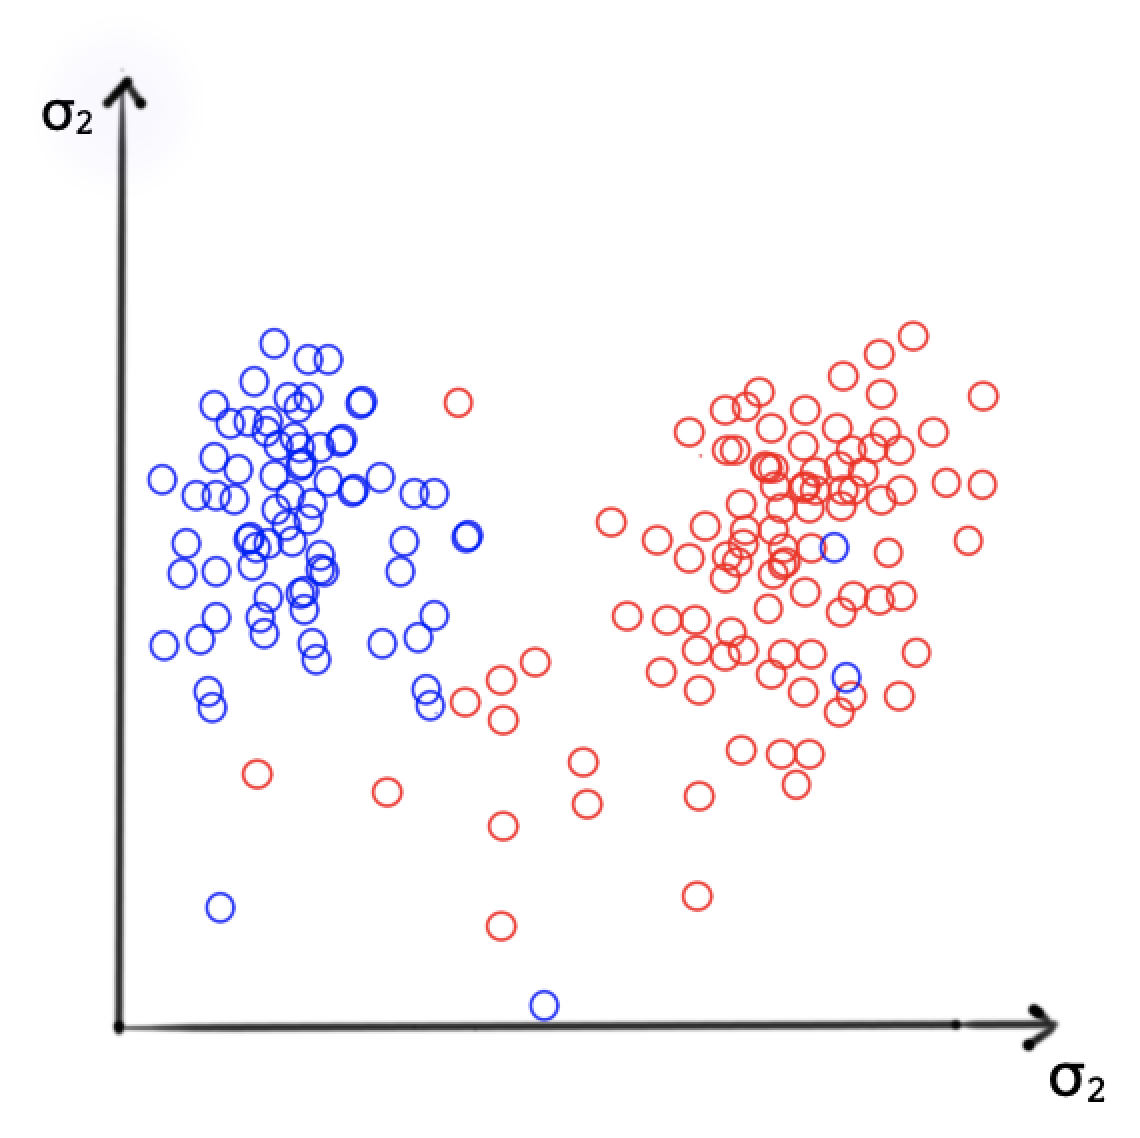
\includegraphics[width=50mm,scale=0.5]{ScreenShot.png}
\end{figure}

\begin{tabular}{p{5cm}c}

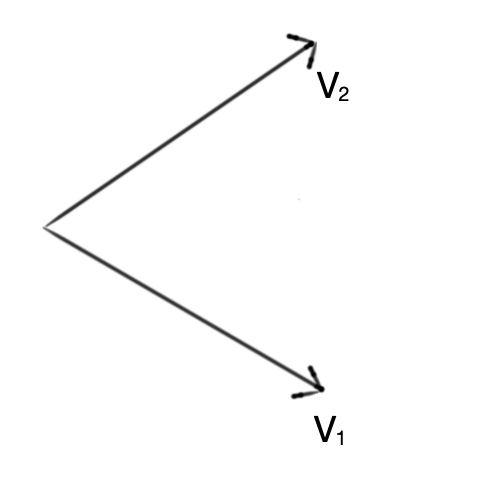
\includegraphics[width=50mm,scale=0.5]{Image002.png}
&
$\begin{pmatrix}
cos\theta & -sin\theta\\
sin\theta& cos\theta    
\end{pmatrix}$= $e^{i\theta}$, \{$e^{i\theta}$\textbar0$\leq\Theta\leq2\pi\}$ = S'

\end{tabular}

\begin{figure}[h!]
  \centering
  \begin{subfigure}[b]{0.3\linewidth}
 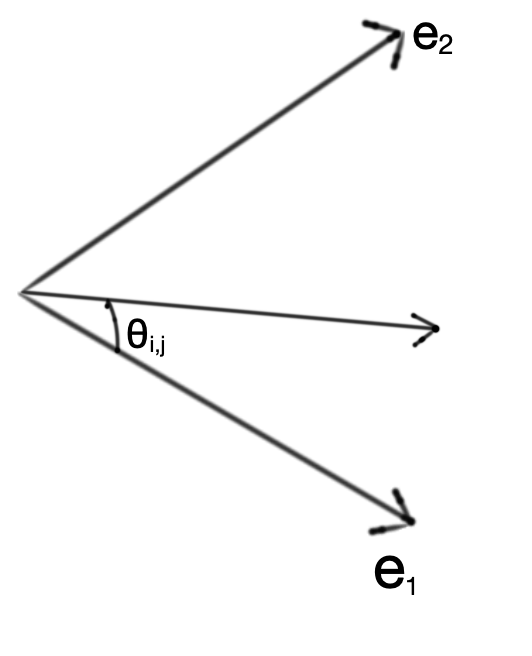
\includegraphics[width=50mm,scale=0.5]{Image003.png}
  \end{subfigure}
 \begin{subfigure}[b]{0.6\linewidth}
    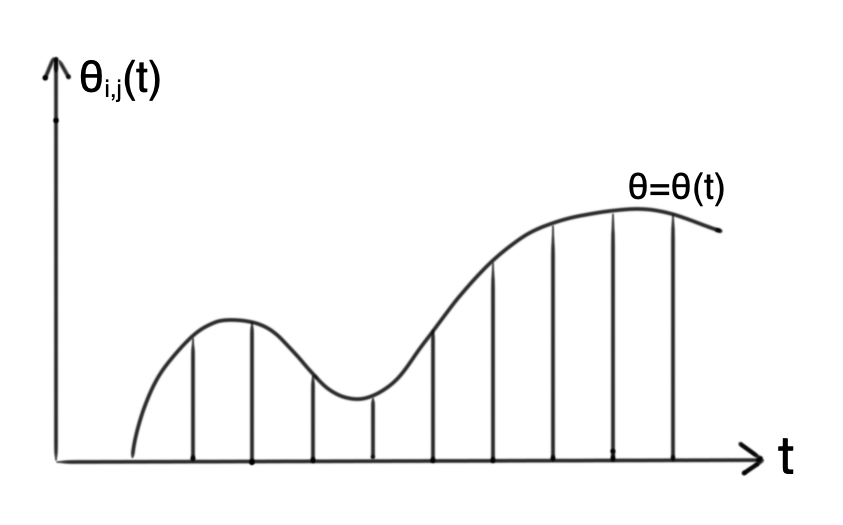
\includegraphics[width=80mm,scale=0.8]{Image004.png}
 
  \end{subfigure}
  
\end{figure}

\end{Large}

\end{document}  